\subsection{Taktgesteuertes RS-Flip-Flop} % (fold)
\label{sub:Taktgesteuertes RS-Flip-Flop}
\begin{frame}
    \frametitle{Taktgesteuertes RS-Flip-Flop}
    \framesubtitle{}
     \begin{figure}[H]
     \begin{center}
             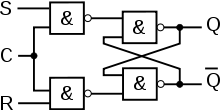
\includegraphics[scale=0.6]{./img/schaltung/RS-FF-T.png}
     \end{center}
     \end{figure}
\end{frame}
\begin{frame}
    \frametitle{Funktionsweise}
    \framesubtitle{}
    \begin{columns}[c]
        \column{0.6\textwidth}
            \boxed{
                \begin{tabular}{c|c|c||c}
                    S & R & C & Q \\
                    \hline
                     0 & 0 & 0 & unverändert \\
                     0 & 1 & 0 & unverändert \\
                     1 & 0 & 0 & unverändert \\
                     1 & 1 & 0 & unverändert \\
                     \hline
                     0 & 0 & 1 & unverändert \\
                     0 & 1 & 1 & 0 (zurückgesetzt) \\
                     1 & 0 & 1 & 1 (gesetzt) \\
                     1 & 1 & 1 & Glitch ($\bar{Q} = Q$)
                \end{tabular}
            }
        \column{0.4\textwidth}
             \begin{figure}[H]
             \begin{center}
                     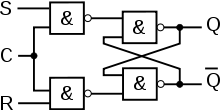
\includegraphics[scale=0.6]{./img/schaltung/RS-FF-T.png}
             \end{center}
             \end{figure}
             \begin{figure}[H]
             \begin{center}
                     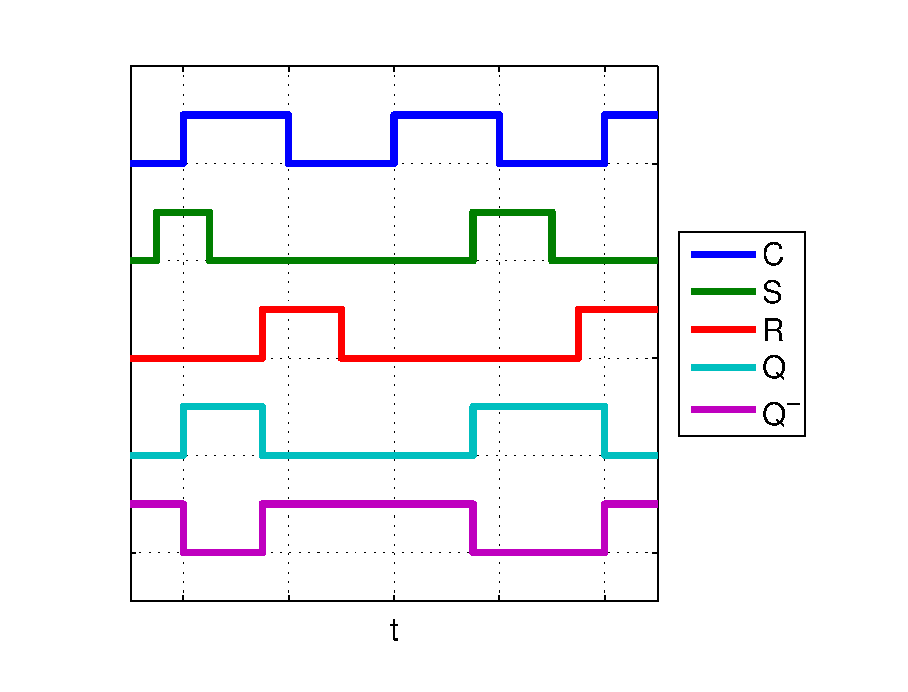
\includegraphics[scale=0.32]{./img/Aufgabe_2_b.eps}
             \end{center}
             \end{figure}
    \end{columns}
\end{frame}
% subsection Taktgesteuertes RS-Flip-Flop (end)
